\documentclass[11pt,a4paper]{article}
\usepackage[english]{babel}
\usepackage[T1]{fontenc}
\usepackage{mathptmx}
\usepackage{amsmath}
\usepackage[a4paper,margin=2.5cm]{geometry}
\usepackage{graphicx}
\usepackage{float}
\usepackage{booktabs}
\usepackage{tabularx}
\usepackage[font=small,labelfont=bf]{caption}
\usepackage{enumitem}
\usepackage{xurl}
\usepackage{tikz}
\usetikzlibrary{arrows.meta,patterns,calc}

\graphicspath{{figures/}}
% generated by evaluation.m - do not edit by hand
\newcommand{\RAluFepsA}{0.447}
\newcommand{\RAluFepsB}{4.333}
\newcommand{\RAluEext}{66.5}
\newcommand{\RAluEmw}{17.8}
\newcommand{\RAluEfak}{3.74}
\newcommand{\RAluFmax}{14.76}
\newcommand{\RAluFbruch}{8.93}
\newcommand{\RAluDbruch}{9.52}
\newcommand{\RAluRm}{227}
\newcommand{\RAluSigB}{138}
\newcommand{\RAluAmw}{14.6}
\newcommand{\RCFKnullFmax}{32.55}
\newcommand{\RCFKnullFzehn}{3.26}
\newcommand{\RCFKnullFfuenfzig}{16.28}
\newcommand{\RCFKnullepsB}{1.504}
\newcommand{\RCFKnullDB}{6.95}
\newcommand{\RCFKnullsigB}{2292}
\newcommand{\RCFKnullEs}{153.5}
\newcommand{\RCFKnullepsBmw}{4.614}
\newcommand{\RCFKnullepsfak}{0.33}
\newcommand{\RCFKnullEmw}{54.6}
\newcommand{\RCFKnullEfak}{2.81}
\newcommand{\RCFKneunzigFmax}{0.54}
\newcommand{\RCFKneunzigFzehn}{0.05}
\newcommand{\RCFKneunzigFfuenfzig}{0.27}
\newcommand{\RCFKneunzigepsB}{0.215}
\newcommand{\RCFKneunzigDB}{0.40}
\newcommand{\RCFKneunzigsigB}{17}
\newcommand{\RCFKneunzigEs}{7.7}
\newcommand{\RCFKneunzigepsBmw}{0.263}
\newcommand{\RCFKneunzigepsfak}{0.82}
\newcommand{\RCFKneunzigEmw}{6.5}
\newcommand{\RCFKneunzigEfak}{1.19}
\newcommand{\RCFKnullneunzigFmax}{32.86}
\newcommand{\RCFKnullneunzigFzehn}{3.29}
\newcommand{\RCFKnullneunzigFfuenfzig}{16.43}
\newcommand{\RCFKnullneunzigepsB}{1.327}
\newcommand{\RCFKnullneunzigDB}{5.10}
\newcommand{\RCFKnullneunzigsigB}{1033}
\newcommand{\RCFKnullneunzigEs}{79.8}
\newcommand{\RCFKnullneunzigepsBmw}{3.297}
\newcommand{\RCFKnullneunzigepsfak}{0.40}
\newcommand{\RCFKnullneunzigEmw}{31.8}
\newcommand{\RCFKnullneunzigEfak}{2.51}
\newcommand{\RGeinsFmaxNullNeunzig}{13.22}
\newcommand{\RGdreiFmaxNeunzig}{1.85}
\newcommand{\RGdreiEpsBNeunzig}{0.571}
\newcommand{\RvAluE}{0.96}
\newcommand{\RvAluB}{5.04}
\newcommand{\RvCFKnull}{5.04}
\newcommand{\RvCFKneunzig}{0.96}
\newcommand{\RvCFKnullneunzig}{5.04}
\newcommand{\PAlub}{16.06}
\newcommand{\PAlut}{4.043}
\newcommand{\PAlutdrei}{4.04 / 4.04 / 4.05}
\newcommand{\PAluL}{65.0}
\newcommand{\PAluA}{64.94}
\newcommand{\PCFKnullb}{16.20}
\newcommand{\PCFKnullt}{0.877}
\newcommand{\PCFKnulltdrei}{0.88 / 0.87 / 0.88}
\newcommand{\PCFKnullL}{150.6}
\newcommand{\PCFKnullA}{14.20}
\newcommand{\PCFKneunzigb}{16.25}
\newcommand{\PCFKneunzigt}{1.917}
\newcommand{\PCFKneunzigtdrei}{1.95 / 1.90 / 1.90}
\newcommand{\PCFKneunzigL}{151.6}
\newcommand{\PCFKneunzigA}{31.15}
\newcommand{\PCFKnullneunzigb}{15.85}
\newcommand{\PCFKnullneunzigt}{2.007}
\newcommand{\PCFKnullneunzigtdrei}{2.00 / 2.00 / 2.02}
\newcommand{\PCFKnullneunzigL}{154.6}
\newcommand{\PCFKnullneunzigA}{31.81}
   % characteristic values from the evaluation script

\newcommand{\eps}{\varepsilon}
\newcommand{\Fmax}{F_{\mathrm{max}}}

\begin{document}

% =====================================================================
% Title page
% =====================================================================
\begin{titlepage}
\centering
{\large Chair of Product Development and Lightweight Design\\
Technical University of Munich\par}
\vspace{2.5cm}
{\LARGE\bfseries Lab Course Report\\[0.3em]
``Scientific Experiment with\\ Research Data Management -- Tensile Test''\par}
\vspace{1cm}
{\large Prof.~Dr.~Markus Zimmermann\\ Winter Semester 2026/2027\par}
\vspace{2.5cm}
\begin{tabular}{|p{6cm}|p{6cm}|}
\hline
\multicolumn{2}{|l|}{\textbf{Group:} 1}\\ \hline
\textbf{Last name:} & \textbf{First name:}\\ \hline
Müller    & Georg   \\ \hline
Qiu       & Junjie  \\ \hline
Radlach   & Mark    \\ \hline
Streicher & Martin  \\ \hline
\end{tabular}
\vfill
{\large Test date: 13.10.2026 \qquad Submission: 27.10.2026\par}
\vspace{0.4cm}
{\small English translation of the report originally submitted in German.\par}
\end{titlepage}

\tableofcontents

\vspace{\baselineskip}

\section*{\small Note on the use of tools:}
{\small The language model Claude (Anthropic) was used as a tool for drafts and evaluation scripts. The structure and tasks of the report follow the assignment of the chair. The report was written in LaTeX. Test execution, specimen dimensions, measurement data and photos are the group's own. All contents, calculations and results were checked and revised by the group, which takes responsibility for them.\par}

\vspace{\baselineskip}

\section*{\small Note on author contributions:}
\begingroup
\small
\begin{tabular}{@{} l p{10cm} @{}}
    \textbf{Georg Müller} & Main author of Sections 1 and 2 (Description of the test objects, Interpretation of the results), plotting of the diagrams, formatting in LaTeX, preparation of the DMP using the TUM template \\
    [1ex]
    \textbf{Junjie Qiu} & Review of the diagrams in Section 1.6 (Plotting) and revision of the CFRP 0° diagrams; support in revising Sections 2.1 (a--b) and 2.2 (a, b, d, e) and adjustment of the corresponding entries in the test protocol \\
    [1ex]
    \textbf{Mark Radlach} & Main author of Section 3 (Test protocol); support for Sections 1.3 (Sources of error), 1.4 (Force measurement) and 1.5 (Strain measurement methods -- transducers) \\
    [1ex]
    \textbf{Martin Streicher} & Review of the calculated results and proofreading \\
\end{tabular}
\endgroup

\newpage

% =====================================================================
\section{Description of the Test Objects}
% =====================================================================

\subsection{Working Principle of the Testing Machine}

The tests were carried out on an electromechanical universal testing machine,
type Instron~4505 (rated force 100\,kN). Figure~\ref{fig:maschine} shows the
basic setup. The load frame consists of a rigid base, two columns, each with a
lead screw, and a fixed upper crosshead. An electric motor in the base drives
both screws synchronously via a gearbox and toothed belt. The screw nuts sit in
the moving crosshead (lower cross member), which therefore moves vertically.

The specimen is clamped between two grips. The upper grip hangs from the fixed
upper crosshead via the load cell, while the lower grip sits on the moving
crosshead. When the crosshead moves down, the specimen is stretched and the
tensile force is measured by the load cell. Since the load cell is mounted on
the fixed crosshead, it does not move; cables and measuring chain stay at rest.
The crosshead travel (crosshead displacement) is recorded by a rotary encoder
on the drive. In addition, the strain can be measured locally on the specimen
with an extensometer or strain gauges. Control and data acquisition run via
the machine electronics and a connected PC; in the test, all channels were
recorded at 100\,Hz.

\begin{figure}[H]
\centering
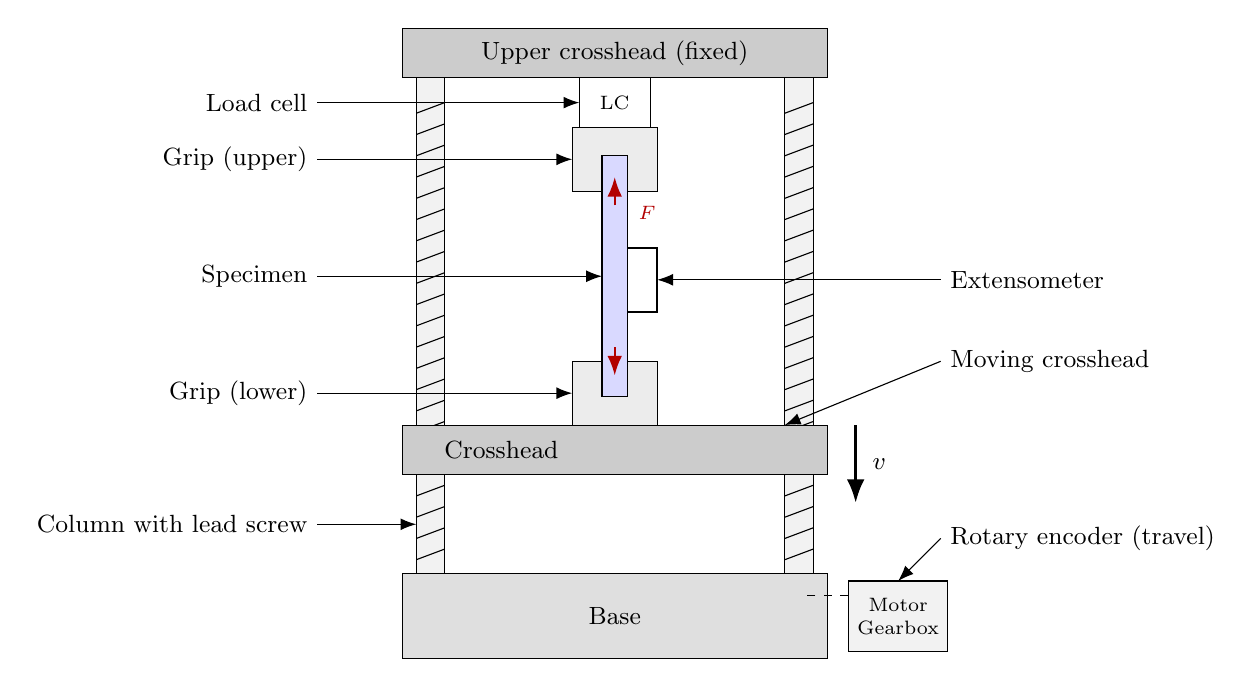
\begin{tikzpicture}[scale=0.9, every node/.style={font=\small},
  lbl/.style={-{Latex[length=2mm]}, thin}]
  % base
  \fill[gray!25] (-3,0) rectangle (3,1.2);
  \draw (-3,0) rectangle (3,1.2);
  \node at (0,0.6) {Base};
  % motor + gearbox
  \draw[fill=gray!10] (3.3,0.1) rectangle (4.7,1.1);
  \node[align=center, font=\scriptsize] at (4.0,0.6) {Motor\\Gearbox};
  \draw[dashed] (3.3,0.9) -- (2.6,0.9);
  % columns with lead screws
  \foreach \x in {-2.6,2.6}{
    \draw[fill=gray!10] (\x-0.2,1.2) rectangle (\x+0.2,8.2);
    \foreach \y in {1.4,1.7,...,8.0} \draw (\x-0.2,\y) -- (\x+0.2,\y+0.15);
  }
  % fixed upper crosshead
  \draw[fill=gray!40] (-3,8.2) rectangle (3,8.9);
  \node at (0,8.55) {Upper crosshead (fixed)};
  % load cell
  \draw[fill=white] (-0.5,7.5) rectangle (0.5,8.2);
  \node[font=\scriptsize] at (0,7.85) {LC};
  % upper grip
  \draw[fill=gray!15] (-0.6,6.6) rectangle (0.6,7.5);
  % moving crosshead
  \draw[fill=gray!40] (-3,2.6) rectangle (3,3.3);
  \node at (-1.6,2.95) {Crosshead};
  \draw[-{Latex[length=3mm]}, very thick] (3.4,3.3) -- (3.4,2.2);
  \node[right] at (3.5,2.75) {$v$};
  % lower grip
  \draw[fill=gray!15] (-0.6,3.3) rectangle (0.6,4.2);
  % specimen
  \draw[fill=blue!15] (-0.18,3.7) rectangle (0.18,7.1);
  % extensometer
  \draw[thick] (0.18,4.9) -- (0.6,4.9) -- (0.6,5.8) -- (0.18,5.8);
  % labels
  \draw[lbl] (-4.2,7.85) node[left]{Load cell} -- (-0.5,7.85);
  \draw[lbl] (-4.2,7.05) node[left]{Grip (upper)} -- (-0.6,7.05);
  \draw[lbl] (-4.2,5.4)  node[left]{Specimen} -- (-0.18,5.4);
  \draw[lbl] (-4.2,3.75) node[left]{Grip (lower)} -- (-0.6,3.75);
  \draw[lbl] (-4.2,1.9)  node[left]{Column with lead screw} -- (-2.8,1.9);
  \draw[lbl] (4.6,5.35)  node[right]{Extensometer} -- (0.6,5.35);
  \draw[lbl] (4.6,4.2)   node[right]{Moving crosshead} -- (2.4,3.3);
  \draw[lbl] (4.6,1.7)   node[right]{Rotary encoder (travel)} -- (4.0,1.1);
  % force flow
  \draw[-{Latex[length=2.5mm]}, red!70!black, thick] (0,6.4) -- (0,6.8);
  \draw[-{Latex[length=2.5mm]}, red!70!black, thick] (0,4.4) -- (0,4.0);
  \node[red!70!black, right, font=\scriptsize] at (0.2,6.3) {$F$};
\end{tikzpicture}
\caption{Schematic of the electromechanical tensile testing machine (Instron~4505).
The lower crosshead is moved down by two lead screws; the load cell (LC) is
mounted on the fixed upper crosshead. The tensile force $F$ flows from the
crosshead through the grips, specimen and LC into the upper crosshead and back
into the base via the columns.}
\label{fig:maschine}
\end{figure}

\subsection{Control, Drive and Clamping}

\paragraph{Control modes.} The drive can be controlled by three quantities:
\begin{itemize}[nosep]
  \item \textbf{Displacement control:} The crosshead moves at constant speed.
        This is the standard case and was also used in the test. The
        measurement data give a testing speed of about \RvAluE\,mm/min for the
        elastic aluminium measurement and the 90\textdegree{} specimen, and
        about \RvAluB\,mm/min for all other tests to fracture.
  \item \textbf{Force control:} The force is increased at a constant rate or
        held at a value (e.\,g.\ for creep or hold phases). After the maximum
        force is reached, this control becomes unstable because the machine
        cannot follow the decreasing force.
  \item \textbf{Strain control:} The controller uses the extensometer signal.
        This sets the strain rate in the specimen directly, independent of the
        compliance of the machine. Some standards for metallic materials
        require this in the range of the proof stress.
\end{itemize}

\paragraph{Drive.} A speed-controlled electric motor drives the two lead
screws via a gearbox and belt, converting the rotation into a linear motion of
the crosshead. Electromechanical drives are very well suited for quasi-static
tests: the speed can be set finely and reproducibly, and there is no hydraulic
system to maintain. For high frequencies (fatigue tests), servo-hydraulic
machines are the better choice.

\paragraph{Clamping (wedge grip principle).} The specimen is held in
mechanical wedge grips (Fig.~\ref{fig:keil}). Two wedges with serrated
clamping faces sit in a housing with an inclined guide. They are first
preloaded by hand. Under the tensile force $F$, the specimen pulls the wedges
deeper into the housing; the incline (wedge angle $\alpha$) creates a normal
force $N$ on the specimen that grows with the tensile force. Neglecting
friction between wedge and housing, approximately
\begin{equation}
  N \approx \frac{F}{2\,\tan\alpha}.
\end{equation}
The clamping is therefore self-reinforcing: the higher the load, the tighter
the grip, as long as the static friction between jaw and specimen
($2\mu N \geq F$) is not exceeded. With CFRP specimens, the serrations of the
jaws would damage the fibres and cause fracture in the grip. The CFRP
specimens therefore have bonded GFRP end tabs that introduce the clamping
force into the specimen over a larger area.

\begin{figure}[H]
\centering
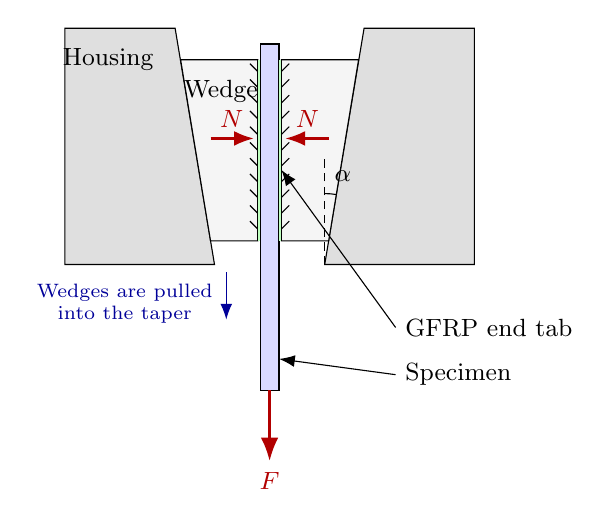
\begin{tikzpicture}[scale=1.0, every node/.style={font=\small}]
  % housing (guide tapers downwards, in pulling direction)
  \fill[gray!25] (-2.6,0) -- (-0.7,0) -- (-1.2,3) -- (-2.6,3) -- cycle;
  \fill[gray!25] (2.6,0) -- (0.7,0) -- (1.2,3) -- (2.6,3) -- cycle;
  \draw (-2.6,0) -- (-0.7,0) -- (-1.2,3) -- (-2.6,3) -- cycle;
  \draw (2.6,0) -- (0.7,0) -- (1.2,3) -- (2.6,3) -- cycle;
  \node at (-2.05,2.6) {Housing};
  % wedges (wider at the top)
  \draw[fill=gray!8] (-0.75,0.3) -- (-0.15,0.3) -- (-0.15,2.6) -- (-1.13,2.6) -- cycle;
  \draw[fill=gray!8] (0.75,0.3) -- (0.15,0.3) -- (0.15,2.6) -- (1.13,2.6) -- cycle;
  \foreach \y in {0.45,0.65,...,2.5}{
    \draw (-0.15,\y) -- (-0.25,\y+0.1);
    \draw (0.15,\y) -- (0.25,\y+0.1);
  }
  \node at (-0.62,2.2) {Wedge};
  % wedge angle
  \draw[densely dashed] (0.7,0) -- (0.7,1.4);
  \draw (0.7,0.9) arc[start angle=90, end angle=80.5, radius=0.9];
  \node at (0.93,1.12) {$\alpha$};
  % wedge motion
  \draw[-{Latex[length=2mm]}, blue!60!black] (-0.55,-0.1) -- (-0.55,-0.7);
  \node[blue!60!black, font=\scriptsize, align=center, left] at (-0.6,-0.5) {Wedges are pulled\\into the taper};
  % specimen with tabs
  \fill[blue!15] (-0.12,-1.6) rectangle (0.12,2.8);
  \draw (-0.12,-1.6) rectangle (0.12,2.8);
  \fill[green!25] (-0.15,0.3) rectangle (-0.12,2.6);
  \fill[green!25] (0.12,0.3) rectangle (0.15,2.6);
  % forces
  \draw[-{Latex[length=3mm]}, very thick, red!70!black] (0,-1.6) -- (0,-2.5)
       node[below] {$F$};
  \draw[-{Latex[length=2.5mm]}, thick, red!70!black] (-0.75,1.6) -- (-0.2,1.6);
  \node[red!70!black, above] at (-0.48,1.62) {$N$};
  \draw[-{Latex[length=2.5mm]}, thick, red!70!black] (0.75,1.6) -- (0.2,1.6);
  \node[red!70!black, above] at (0.48,1.62) {$N$};
  % labels
  \draw[-{Latex[length=2mm]}, thin] (1.6,-0.8) node[right]{GFRP end tab} -- (0.15,1.2);
  \draw[-{Latex[length=2mm]}, thin] (1.6,-1.4) node[right]{Specimen} -- (0.12,-1.2);
\end{tikzpicture}
\caption{Wedge grip of the upper grip (section; the lower one is mirrored).
The tensile force $F$ pulls the wedges into the conical guide, so that the
normal force $N$ on the specimen also increases with the load.}
\label{fig:keil}
\end{figure}

\subsection{Sources of Error}

\begin{enumerate}[label=(\alph*)]
\item \textbf{Possible errors during the test or caused by the testing machine}
\begin{itemize}[nosep]
  \item \emph{Machine compliance:} The load frame, screws, load cell and grips
        also deform elastically. The crosshead displacement contains this
        deformation and clearly overestimates the specimen strain.
  \item \emph{Seating and slipping in the grips:} The wedges settle at the
        start of the test and the serrations press into the specimen or end
        tab. This appears as a non-linear initial region of the
        force--displacement curve (e.\,g.\ Fig.~\ref{fig:b}).
  \item \emph{Deformation outside the gauge length:} Specimen, end tabs and
        adhesive layer between the grips also stretch; the reference length
        for the crosshead displacement is therefore not clearly defined.
  \item \emph{Misalignment:} If the grips are not exactly coaxial or the
        specimen is clamped at an angle, bending stresses occur in addition to
        the intended uniaxial loading. These distort the strain measurement
        and can cause premature fracture.
  \item \emph{Failure of the load introduction:} Fracture in the grip or
        debonding of the end tabs. Both occurred in Group~1 (90\textdegree{}
        and 0\textdegree/90\textdegree{} specimen, see
        Section~\ref{sec:plotten}).
  \item \emph{Sensor errors:} misaligned or poorly bonded strain gauges,
        temperature drift, slipping of the extensometer knife edges, zero
        offsets of the channels.
  \item \emph{Geometry:} Measurement inaccuracy in width and thickness enters
        stress and Young's modulus directly; thickness variations are
        particularly relevant for CFRP.
  \item \emph{Environment and testing speed:} Temperature and humidity mainly
        affect the matrix; an excessive testing speed changes the
        characteristic values.
\end{itemize}

\item \textbf{Remedies}
\begin{itemize}[nosep]
  \item Measure strain locally on the specimen (extensometer, strain gauges)
        instead of via the crosshead displacement, or subtract the machine
        compliance using a calibration test.
  \item Determine Young's modulus between two limits rather than from zero
        (0.01\,\%/0.1\,\% strain for aluminium, 10\,\%/50\,\% $\Fmax$ for
        CFRP). This removes seating and zero-point errors.
  \item Apply a small preload before the measurement starts.
  \item Align the grips and clamp the specimen centrally; if needed, apply
        strain gauges on front and back to check for bending.
  \item Bond end tabs carefully (surface preparation, full curing), use
        chamfered tabs to reduce stress peaks; discard specimens that break
        in the grip.
  \item Measure specimen dimensions at several points with a micrometer and
        average; test at least five specimens per variant.
  \item Calibrate the load cell and maintain the test equipment regularly.
  \item Keep to and document the standard atmosphere and the prescribed
        testing speed.
  \item When clamping the AlMg3 specimen, use a prefabricated jig that allows
        nearly uniaxial positioning centred in the jaws. Alternatively, and
        for the CFRP specimens, calculate the central position from the jaw
        and specimen geometry at the top and bottom and measure it with a
        caliper.
\end{itemize}
\end{enumerate}

\subsection{Force Measurement}

The force is measured with a strain-gauge-based load cell. It consists of a
metallic spring element that sits in the force flow between the fixed
crosshead and the upper grip and deforms elastically and in proportion to the
force under load. Strain gauges are applied to the spring element and wired as
a Wheatstone full bridge: two gauges are stretched, two compressed (or
stretched transversely). The relative change in resistance
$\Delta R/R = k\,\eps$ ($k\approx 2$) leads to a bridge output
\begin{equation}
  \frac{U_A}{U_B} = \frac{k}{4}\,(\eps_1 - \eps_2 + \eps_3 - \eps_4),
\end{equation}
which is amplified and digitised. Compared with a single gauge, the full
bridge doubles or quadruples the signal and compensates for temperature
effects as well as bending and transverse forces. The load cell is calibrated
against reference weights or a standard; the output voltage is then directly
proportional to the force.

\subsection{Strain Measurement Methods -- Transducers}

Three methods were used in the test. Table~\ref{tab:sensoren} summarises them.

\paragraph{Strain gauges (SG).} A meander-shaped metal foil grid on a carrier
film is bonded to the specimen and stretches with it. Its electrical
resistance changes in proportion to the strain ($\Delta R/R = k\,\eps$).
Since the relative change in resistance is very small, only the resulting
voltage change is recorded using a Wheatstone bridge circuit. Strain gauges
were used on the CFRP~0\textdegree{} and CFRP~0\textdegree/90\textdegree{}
specimens.

\paragraph{Extensometer.} Two knife edges are clamped to the specimen at the
initial gauge length $l_0$ (12.5, 25 or 50\,mm). If their distance changes, a
flexible beam in the housing deforms, whose strain is in turn measured with
strain gauges. Measuring range $\pm 5$\,mm, resolution about $10^{-5}$.
Because the extensometer is fragile and expensive, it was only used in tests
with clearly lower fracture energy: in Test~1 on the AlMg3 specimen to
determine Young's modulus, and in Test~4 on the CFRP UD 90\textdegree{}
specimen to fracture.

\paragraph{Crosshead displacement.} The crosshead travel is recorded without
an additional sensor and related to a reference length. It contains all
deformations in the force flow and is therefore only suitable as a rough
approximation.

\begin{table}[H]
\centering
\caption{Comparison of the strain transducers (costs as order of magnitude).}
\label{tab:sensoren}
\small
\begin{tabularx}{\textwidth}{@{}l>{\raggedright}X>{\raggedright}X>{\raggedright\arraybackslash}X@{}}
\toprule
 & \textbf{Strain gauge} & \textbf{Extensometer} & \textbf{Crosshead displacement}\\
\midrule
Principle & Change in resistance of a bonded measuring grid &
  Change in distance between two knife edges, measured via strain gauges on a flexure beam &
  Rotary encoder on the drive, crosshead travel \\
Cost & a few to several tens of \texteuro\ per gauge, plus adhesive,
  wiring and application time; single use &
  several thousand \texteuro, but reusable & no additional cost \\
Advantages & very accurate, local, measures up to fracture, even at high
  fracture energy & quick to attach, reusable, averages over $l_0$ &
  always available, unlimited measuring range \\
Disadvantages & time-consuming application, local only, not
  reusable, limited measuring range & can be damaged by high-energy
  fracture, knife edges can slip & includes machine and grip deformation,
  large errors \\
\bottomrule
\end{tabularx}
\end{table}

\subsection{Plotting}
\label{sec:plotten}

The measurement data were imported, evaluated and plotted with the MATLAB
script \texttt{evaluation.m} (based on the import script provided by the chair).
The evaluation points from Section~\ref{sec:auswerten} are marked
accordingly. For CFRP~0\textdegree{}, the red dot marks the maximum force; in
the other fracture diagrams it marks the selected fracture point. The limits
of the Young's modulus determination are shown as green dashed lines. The
CFRP~0\textdegree{} diagrams also include the data after the maximum force;
this time interval is shown as a grey dashed line.

\paragraph{Particularities of the Group~1 measurements.}
The CFRP 0\textdegree/90\textdegree{} specimen of Group~1 could not be tested
to fracture because the bond of a GFRP end tab failed prematurely and the tab
slipped off (Fig.~\ref{fig:foto_cfk090}). The force only rose to about
\RGeinsFmaxNullNeunzig\,kN and then decreased gradually as the tab debonded.
As instructed, the evaluation uses the measurement data of the
0\textdegree/90\textdegree{} specimen of Group~3 (fracture at
\RCFKnullneunzigFmax\,kN); the Group~1 curve is shown in grey in
Fig.~\ref{fig:h} and~\ref{fig:i} for documentation.

The 90\textdegree{} specimen of Group~1 broke in the grip area at only
\RCFKneunzigFmax\,kN (Group~3: \RGdreiFmaxNeunzig\,kN). A fracture outside the
gauge length does not reflect the material behaviour; the strength and
elongation at break of this specimen are therefore of limited validity. The
Group~3 curve is shown in grey for comparison.

\newcommand{\plot}[4][]{%
\begin{figure}[H]\centering
\includegraphics[width=0.78\textwidth,#1]{#2}
\caption{#3}\label{#4}
\end{figure}}

\plot{a_alu_elast_ext}{(a) AlMg3 elastic: force vs.\ extensometer strain.
Limits of the Young's modulus determination at $\eps = 0.01\,\%$ and $0.1\,\%$.}{fig:a}
\plot{b_alu_elast_mw}{(b) AlMg3 elastic: force vs.\ crosshead displacement.
The forces at $\eps = 0.01\,\%$ and $0.1\,\%$ (extensometer) are transferred
as limits.}{fig:b}
\plot{c_alu_bruch_mw}{(c) AlMg3 fracture: force vs.\ crosshead displacement with
maximum force $\Fmax$ and fracture point.}{fig:c}
\plot{de_cfk0_full_eps}{(d) CFRP~0\textdegree{}:
force vs.\ strain gauge strain with the complete measurement. Blue: up to the
maximum force; grey dashed: afterwards. The red dot marks the maximum
force.}{fig:d}
\plot{de_cfk0_full_mw}{(e) CFRP~0\textdegree{}:
force vs.\ crosshead displacement with the complete measurement. Blue: up to
the maximum force; grey dashed: afterwards. The red dot marks the maximum
force.}{fig:e}
\plot{fg_cfk90_eps}{(f) CFRP~90\textdegree{}: force vs.\ extensometer strain (Group~1,
fracture in the grip; Group~3 for comparison).}{fig:f}
\plot{fg_cfk90_mw}{(g) CFRP~90\textdegree{}: force vs.\ crosshead displacement.}{fig:g}
\plot{hi_cfk090_eps}{(h) CFRP 0\textdegree/90\textdegree{}: force vs.\ strain gauge strain (evaluated:
Group~3; Group~1 with end tab failure in grey).}{fig:h}
\plot{hi_cfk090_mw}{(i) CFRP 0\textdegree/90\textdegree{}: force vs.\ crosshead displacement.}{fig:i}

% =====================================================================
\section{Interpretation of the Results}
% =====================================================================

\subsection{Evaluation}
\label{sec:auswerten}

The evaluation is based on the specimen dimensions from the test protocol
(Table~\ref{tab:protokoll}). For the 0\textdegree/90\textdegree{} specimen, the
measurement data of Group~3 are used together with the dimensions of the
identical specimen from our own protocol; differences in cross-section between
the two specimens therefore enter stress and Young's modulus directly. The
initial cross-section is $A_0 = b\cdot t$; the strain from the crosshead
displacement is calculated as $\eps_{\mathrm{CH}} = \Delta l / L_0$ with the
reference length $L_0$.

\begin{enumerate}[label=(\alph*)]
\item \textbf{Fracture stress.} The fracture stress follows from the fracture
force and the initial cross-section, $\sigma_B = F_B/A_0$. For the
CFRP~0\textdegree{} specimen, the maximum nominal stress is determined from
the maximum force. After $\Fmax = \RCFKnullFmax$\,kN is reached, a
considerable load-bearing capacity initially remains. The maximum force point
is therefore distinguished from the later complete force drop. For AlMg3, the
tensile strength $R_m = \Fmax/A_0$ and the stress at the fracture point
$F_B/A_0$ are given separately, since the force decreases after necking until
fracture. The fracture points are marked in Fig.~\ref{fig:c}, \ref{fig:f}
and~\ref{fig:h}; for CFRP~0\textdegree{}, the maximum force point is marked in
Fig.~\ref{fig:d} and~\ref{fig:e}.

\begin{table}[H]
\centering
\caption{Fracture forces and fracture stresses.}
\label{tab:bruch}
\begin{tabular}{@{}lcccc@{}}
\toprule
Specimen & $\Fmax$ [kN] & $F_B$ [kN] & $A_0$ [mm$^2$] & $\sigma_B$ [N/mm$^2$]\\
\midrule
AlMg3 & \RAluFmax & \RAluFbruch & \PAluA & $R_m$ = \RAluRm;\ \RAluSigB\\
CFRP UD 0\textdegree & \RCFKnullFmax & \RCFKnullFmax & \PCFKnullA & \RCFKnullsigB\\
CFRP UD 90\textdegree$^{*}$ & \RCFKneunzigFmax & \RCFKneunzigFmax & \PCFKneunzigA & \RCFKneunzigsigB\\
CFRP 0\textdegree/90\textdegree$^{**}$ & \RCFKnullneunzigFmax & \RCFKnullneunzigFmax & \PCFKnullneunzigA & \RCFKnullneunzigsigB\\
\bottomrule
\multicolumn{5}{@{}l}{\footnotesize $^{*}$ Fracture in the grip, limited validity.\quad
$^{**}$ Measurement data of Group~3.}
\end{tabular}
\par\smallskip
\noindent\parbox{\linewidth}{\footnotesize CFRP~0\textdegree{}:
The force, stress, strain and displacement values refer to the maximum force
point. Fracture force and elongation at break were not determined
independently of it.}
\end{table}

\item \textbf{Elongation at break of the CFRP specimens.} The strain and
displacement values are read at the marked evaluation point from the strain
gauge or extensometer and the crosshead displacement
(Fig.~\ref{fig:d}--\ref{fig:i}). For CFRP~0\textdegree{}, the values refer to
the maximum force point: $\eps(\Fmax) = \RCFKnullepsB\,\%$ and
$\Delta l(\Fmax) = \RCFKnullDB$\,mm. No independently determined elongation at
break is given for this specimen. The error factor is
$f_\eps = \eps_{\mathrm{SG/Ext}}/\eps_{\mathrm{CH}}$.

\begin{table}[H]
\centering
\caption{Elongation at break of the CFRP specimens and error factor.}
\label{tab:dehnung}
\begin{tabular}{@{}lccccc@{}}
\toprule
Specimen & $\eps_{B,\mathrm{SG/Ext}}$ [\%] & $\Delta l_B$ [mm] & $L_0$ [mm] &
$\eps_{B,\mathrm{CH}}$ [\%] & $f_\eps$ [--]\\
\midrule
CFRP UD 0\textdegree & \RCFKnullepsB & \RCFKnullDB & \PCFKnullL & \RCFKnullepsBmw & \RCFKnullepsfak\\
CFRP UD 90\textdegree$^{*}$ & \RCFKneunzigepsB & \RCFKneunzigDB & \PCFKneunzigL & \RCFKneunzigepsBmw & \RCFKneunzigepsfak\\
CFRP 0\textdegree/90\textdegree$^{**}$ & \RCFKnullneunzigepsB & \RCFKnullneunzigDB & \PCFKnullneunzigL & \RCFKnullneunzigepsBmw & \RCFKnullneunzigepsfak\\
\bottomrule
\end{tabular}
\par\smallskip
\noindent\parbox{\linewidth}{\footnotesize CFRP~0\textdegree{}:
The force, stress, strain and displacement values refer to the maximum force
point. Fracture force and elongation at break were not determined
independently of it.}
\end{table}

The error factor is smaller than one, so the strain from the crosshead
displacement is larger than the actual specimen strain. Besides the
elongation of the specimen within the gauge length, the crosshead displacement
also contains the elastic deformation of the load frame, screws, load cell and
grips, the seating and slipping of the wedges, the deformation of the end tabs
and adhesive layers, and the strain of the specimen outside the gauge length.
All of these contributions are wrongly attributed to the reference length.
Strain gauges and extensometer, in contrast, measure directly on the specimen.

\item \textbf{Young's modulus.} For AlMg3, Young's modulus is determined
between the strain limits $\eps_{0.01} = 0.01\,\%$ and $\eps_{0.1} = 0.1\,\%$
(Fig.~\ref{fig:a}, \ref{fig:b}):
\begin{equation}
E = \frac{F_{\eps 0.1} - F_{\eps 0.01}}{A_0\,(\eps_{0.1} - \eps_{0.01})}
  = \frac{F_{\eps 0.1} - F_{\eps 0.01}}{A_0 \cdot 0.09\,\%},
\end{equation}
with $F_{\eps 0.01} = \RAluFepsA$\,kN and $F_{\eps 0.1} = \RAluFepsB$\,kN.
For the CFRP specimens, the secant modulus between 10\,\% and 50\,\% of the
fracture force is determined according to EN~2561
(Fig.~\ref{fig:d}--\ref{fig:i}):
\begin{equation}
E = \frac{F_{50} - F_{10}}{A_0\,(\eps_{F50} - \eps_{F10})}
  = \frac{0.4\,\Fmax}{A_0\,(\eps_{F50} - \eps_{F10})}.
\end{equation}
For the crosshead displacement, the same force limits are used and the
strains are replaced by $\Delta l/L_0$. The error factor is
$f_E = E_{\mathrm{SG/Ext}}/E_{\mathrm{CH}}$.

\begin{table}[H]
\centering
\caption{Young's moduli and error factor.}
\label{tab:emodul}
\begin{tabular}{@{}lcccc@{}}
\toprule
Specimen & Limits & $E_{\mathrm{SG/Ext}}$ [GPa] & $E_{\mathrm{CH}}$ [GPa] & $f_E$ [--]\\
\midrule
AlMg3 & 0.01--0.1\,\% $\eps$ & \RAluEext & \RAluEmw & \RAluEfak\\
CFRP UD 0\textdegree & \RCFKnullFzehn--\RCFKnullFfuenfzig\,kN & \RCFKnullEs & \RCFKnullEmw & \RCFKnullEfak\\
CFRP UD 90\textdegree$^{*}$ & \RCFKneunzigFzehn--\RCFKneunzigFfuenfzig\,kN & \RCFKneunzigEs & \RCFKneunzigEmw & \RCFKneunzigEfak\\
CFRP 0\textdegree/90\textdegree$^{**}$ & \RCFKnullneunzigFzehn--\RCFKnullneunzigFfuenfzig\,kN & \RCFKnullneunzigEs & \RCFKnullneunzigEmw & \RCFKnullneunzigEfak\\
\bottomrule
\end{tabular}
\end{table}

The error factor $f_E$ is larger than one: the modulus from the crosshead
displacement is too low because the denominator contains the same excessive
strain as in~(b). Since only a force interval is considered here, zero-point
and seating errors are largely eliminated; the compliance of the machine,
grips and end tabs, however, remains fully included. The stiffer the specimen
relative to the machine, the larger the error. The values confirm this: $f_E$
is largest for the thick aluminium specimen (\RAluEfak), followed by
CFRP~0\textdegree{} (\RCFKnullEfak) and 0\textdegree/90\textdegree{}
(\RCFKnullneunzigEfak); for the very compliant 90\textdegree{} specimen it is
smallest at \RCFKneunzigEfak.
\end{enumerate}

\subsection{Comparison and Assessment of the Material Specimens}

The reference values are the manufacturer data of the prepreg system KUBD~1409
(UTS fibre, epoxy resin, fibre volume fraction approx.\ 60\,\%):
$E_{0} \approx 148$\,GPa, $R_{0} \approx 2100$\,N/mm$^2$,
$\eps_{B,0} \approx 1\,\%$; $E_{90} \approx 9$\,GPa,
$R_{90} \approx 34$\,N/mm$^2$, $\eps_{B,90} \approx 0.4$--$0.5\,\%$.

\begin{enumerate}[label=(\alph*)]
\item \textbf{Young's modulus of the CFRP specimens.} The measured values are
$E_{0} = \RCFKnullEs$\,GPa, $E_{0/90} = \RCFKnullneunzigEs$\,GPa and
$E_{90} = \RCFKneunzigEs$\,GPa. The order $E_{0} > E_{0/90} > E_{90}$ follows
from the load distribution. In the 0\textdegree{} specimen, all fibres are
aligned with the load and the stiffness is fibre-dominated. In the
90\textdegree{} specimen, the fibres are transverse and the load has to be
carried by the matrix and the fibre--matrix interface; the stiffness is
matrix-dominated and about one order of magnitude lower. The laminate
$[0/90/0/90/0]_\mathrm{s}$ contains six 0\textdegree{} and four
90\textdegree{} plies. A simple rule of mixtures over the ply fractions gives
an expected value of about $0.6 \cdot 148 + 0.4 \cdot 9 \approx 92$\,GPa. Here
too, the 0\textdegree{} fibres dominate. $E_0$ agrees well with the
manufacturer value, $E_{90}$ is slightly lower. The somewhat lower value of the
laminate could be related, among other things, to a different fibre volume
fraction. A higher resin content lowers the fibre volume fraction and thus
the stiffness, all else being equal. Whether this is actually the cause for
the tested specimen cannot be concluded from the greater thickness alone. In
addition, the measurement data and specimen dimensions come from different
specimens.

\item \textbf{Elongation at break of the CFRP specimens.} The measured values
are $\eps_0(\Fmax) = \RCFKnullepsB\,\%$,
$\eps_{B,0/90} = \RCFKnullneunzigepsB\,\%$ and
$\eps_{B,90} = \RCFKneunzigepsB\,\%$ (Group~3: \RGdreiEpsBNeunzig\,\%). For
CFRP~0\textdegree{}, a strain of $\RCFKnullepsB\,\%$ was measured at the
maximum force point. Since a considerable load-bearing capacity remains
afterwards, this value is not simply equated with the fibre elongation at
break. At 90\textdegree{}, the matrix or the fibre--matrix interface fails at
low strain (matrix-dominated). Because of the fracture in the grip, the
Group~1 value is clearly below the expected range, while the Group~3 value is
within it. In the 0\textdegree/90\textdegree{} laminate, the 90\textdegree{}
plies crack first (inter-fibre fracture at about the elongation at break of
the 90\textdegree{} specimen), but the laminate continues to carry load via
the 0\textdegree{} plies. The elongation at break of the laminate is therefore
determined by the fibres and is of the same order as that of the
0\textdegree{} specimen.

\item \textbf{Young's modulus of AlMg3 compared with CFRP.} For AlMg3,
$E = \RAluEext$\,GPa (literature approx.\ 70\,GPa). As expected, the value is
clearly below $E_{0}$ and $E_{0/90}$, but far above $E_{90}$. Aluminium is
isotropic: its stiffness is the same in all directions, whereas CFRP is
stiffer only in the fibre direction. Relative to density
($\rho_{\mathrm{Al}} \approx 2.7$\,g/cm$^3$,
$\rho_{\mathrm{CFRP}} \approx 1.5$--$1.6$\,g/cm$^3$), the advantage of CFRP in
the fibre direction is even greater. \emph{Conclusion:} CFRP makes sense when
the main load directions are known and the fibres can be aligned accordingly,
e.\,g.\ in tension struts, spars or pressure vessels. For multiaxial,
changing or unknown load directions, at load introduction points, and where
damage tolerance and reparability are important, aluminium is often the
simpler and more robust choice. A quasi-isotropic CFRP laminate has a
stiffness of the same order as aluminium but is considerably lighter.

\item \textbf{Tensile strength of AlMg3 and CFRP.} The measured values are
$R_{m,\mathrm{Al}} = \RAluRm$\,N/mm$^2$, $\sigma_{B,0} = \RCFKnullsigB$\,N/mm$^2$,
$\sigma_{B,0/90} = \RCFKnullneunzigsigB$\,N/mm$^2$ and
$\sigma_{B,90} = \RCFKneunzigsigB$\,N/mm$^2$. $R_{m,\mathrm{Al}}$ matches the
literature value of about 225\,N/mm$^2$; $\sigma_{B,0}$ is slightly above the
manufacturer value of 2100\,N/mm$^2$. Because of the fracture in the grip,
$\sigma_{B,90}$ is only about half the manufacturer value (34\,N/mm$^2$) and
is not representative. Fibre orientation has a very large influence in CFRP:
in the fibre direction, the strength exceeds that of AlMg3 many times over,
while transverse to it, it is far lower because failure is mainly governed by
the matrix and the fibre--matrix interface. The 0\textdegree/90\textdegree{}
laminate lies in between, roughly according to the fraction of 0\textdegree{}
plies. A quasi-isotropic laminate (e.\,g.\ $[0/\pm45/90]_\mathrm{s}$) has more
direction-independent properties and reaches about the strength of
high-strength aluminium alloys at a lower density. Unlike aluminium, however,
CFRP fails in a brittle manner without plastic reserve and is sensitive to
impact and notches. Aluminium yields before fracture and reduces stress peaks
through plastic flow.

\item \textbf{Fracture patterns and failure modes.}
\begin{itemize}[nosep]
  \item \emph{AlMg3 (Fig.~\ref{fig:foto_alu}):} ductile failure. The curve
        (Fig.~\ref{fig:c}) shows a linear elastic region, yielding with strain
        hardening up to $\Fmax$, then necking with decreasing force and
        finally fracture. The photos show the clear local necking in width and
        thickness and a fracture surface inclined to the load direction
        (shear fracture in the necking zone). In the clamping area, the marks
        of the serrated jaws are visible; the specimen is undeformed there.
  \item \emph{CFRP~0\textdegree{} (Fig.~\ref{fig:foto_cfk0}):} brittle,
        fibre-dominated failure. The curve is almost linear up to the maximum
        force point (Fig.~\ref{fig:d}). Small force drops are visible; their
        exact cause cannot be determined from the measurement signals alone.
        After the maximum force, a considerable load-bearing capacity
        initially remains before the force drops to almost zero. Fracture
        occurred suddenly with a high release of energy: the specimen split
        longitudinally into individual fibre bundles and strips over its
        entire free length (``broom-like fracture''). The splits are caused by
        matrix cracks parallel to the fibres, which dissipate the released
        energy. The end tabs remained intact.
  \item \emph{CFRP~90\textdegree:} brittle, matrix-dominated failure at low
        force and without warning; the curve (Fig.~\ref{fig:f}) is almost
        linear up to fracture. Such an inter-fibre fracture typically runs
        smoothly and perpendicular to the load direction between the fibres.
        In Group~1, the fracture occurred in the grip; no photo of the
        fracture pattern is available.
  \item \emph{CFRP~0\textdegree/90\textdegree{} (Fig.~\ref{fig:foto_cfk090}):}
        In Group~1, the specimen did not break; instead, a GFRP end tab
        slipped off. The bond between tab and specimen failed; adhesive
        residue is visible on the specimen surface and on the edge of the tab,
        while the specimen itself is undamaged. In the diagram, this shows as
        a gradual force drop after about \RGeinsFmaxNullNeunzig\,kN instead of
        a sudden fracture (Fig.~\ref{fig:h}). With regular failure (Group~3),
        the curve is almost linear up to fracture; the inter-fibre fractures
        of the 90\textdegree{} plies reduce the stiffness only slightly, as the
        0\textdegree{} plies carry the load. The final failure is a brittle
        fibre fracture with delaminations between the plies.
\end{itemize}
\end{enumerate}

\newcommand{\foto}[2]{\includegraphics[height=#1]{photos/#2}}

\begin{figure}[H]
\centering
\foto{6.2cm}{alu_bruch_einspannung}\hfill
\foto{6.2cm}{alu_bruch_seite}\hfill
\foto{6.2cm}{alu_bruch_hand}
\caption{AlMg3 after fracture: left and centre still clamped, with necking and
inclined fracture surface; right, one specimen half with jaw marks in the
clamping area.}
\label{fig:foto_alu}
\end{figure}

\begin{figure}[H]
\centering
\foto{8cm}{cfk0_bruch_gesamt}\hspace{0.5cm}
\foto{8cm}{cfk0_bruch_detail}
\caption{CFRP UD 0\textdegree{} after fracture: specimen split into fibre
bundles over its entire free length (``broom-like fracture''), detail on the
right.}
\label{fig:foto_cfk0}
\end{figure}

\begin{figure}[H]
\centering
\foto{7cm}{cfk090_probe}\hspace{0.6cm}
\foto{7cm}{cfk090_aufleimer_oben}\hspace{0.6cm}
\foto{7cm}{cfk090_aufleimer_seite}
\caption{CFRP 0\textdegree/90\textdegree{} of Group~1: left, the unbroken
specimen with strain gauge; centre and right, the slipped GFRP end tab with
adhesive residue (front and side view).}
\label{fig:foto_cfk090}
\end{figure}

% =====================================================================
\section{Test Protocol}
% =====================================================================

\begin{table}[H]
\centering
\caption{Specimen dimensions and sensors. Thickness measured top/centre/bottom, $\bar t$ mean value.}
\label{tab:protokoll}
\small
\begin{tabular}{@{}clccccl@{}}
\toprule
No. & Material & $b$ [mm] & Thickness [mm] & $\bar t$ [mm] & $L_0$ [mm] & Sensors\\
\midrule
1 & AlMg3 & \PAlub & \PAlutdrei & \PAlut & \PAluL & Extensometer, crosshead\\
3 & CFRP UD 0 & \PCFKnullb & \PCFKnulltdrei & \PCFKnullt & \PCFKnullL & SG, crosshead\\
4 & CFRP UD 90 & \PCFKneunzigb & \PCFKneunzigtdrei & \PCFKneunzigt & \PCFKneunzigL & Extensometer, crosshead\\
5 & CFRP 0/90$^{**}$ & \PCFKnullneunzigb & \PCFKnullneunzigtdrei & \PCFKnullneunzigt & \PCFKnullneunzigL & SG, crosshead\\
\bottomrule
\end{tabular}
\end{table}

\begin{table}[H]
\centering
\caption{Notes, events and fracture pattern.}
\small
\begin{tabularx}{\textwidth}{@{}c>{\raggedright\arraybackslash}X@{}}
\toprule
No. & Notes / events / fracture pattern / other\\
\midrule
1 & AlMg3 specimen purely elastic with calibrated extensometer up to approx.\ 7\,kN (approx.\ \RvAluE\,mm/min).\\
2 & Load on AlMg3 specimen reduced to 60\,N in manual mode. Extensometer removed. Crosshead displacement zeroed again. Displacement-controlled at constant speed to fracture (approx.\ \RvAluB\,mm/min). $\Fmax = \RAluFmax$\,kN. Fracture pattern as expected: necking and inclined fracture surface (Fig.~\ref{fig:foto_alu}).\\
3 & CFRP UD 0\textdegree{} specimen with strain gauge, displacement-controlled to fracture (approx.\ \RvCFKnull\,mm/min). Maximum force of
    \RCFKnullFmax\,kN at 101.34\,s. A considerable load-bearing capacity then remains for about four seconds; between
    105.52\,s and 105.53\,s the force drops to almost zero. Fracture pattern: specimen heavily split in the longitudinal direction. GFRP end tabs intact (Fig.~\ref{fig:foto_cfk0}).\\
4 & CFRP UD 90\textdegree{} specimen with extensometer, displacement-controlled to fracture (approx.\ \RvCFKneunzig\,mm/min). Fracture in the grip area at \RCFKneunzigFmax\,kN; approx.\ 1\,kN was expected. The test is therefore of limited validity and would have to be repeated. Due to time constraints, we continued with the next test. No photo of the fracture pattern available.\\
5 & CFRP 0/90 specimen with strain gauge to fracture (approx.\ 5\,mm/min). Group~1 had two faulty test runs. First, the specimen was not clamped firmly enough, so the force decreased during the test while the crosshead displacement increased. The specimen was therefore unloaded in manual mode, preloaded again and the crosshead displacement zeroed again. The test was then restarted at the same speed.
The same faulty behaviour was observed, after which the test was stopped and the specimen inspected: GFRP end tab slipped at \RGeinsFmaxNullNeunzig\,kN (bond failed, Fig.~\ref{fig:foto_cfk090}), no fracture of the specimen. Evaluation with the data of Group~3 (fracture at \RCFKnullneunzigFmax\,kN).\\
\bottomrule
\end{tabularx}
\end{table}

% =====================================================================
\appendix
\section{Data Management Plan}
% =====================================================================

\subsection*{DMP submitted by}
Group~1: Georg Müller, Junjie Qiu, Mark Radlach, Martin Streicher,
Technical University of Munich

\subsection*{Submitted on}
27.10.2026

\subsection*{Project name}
Tensile test: test execution and research data management

\subsection*{Formal context of the project}
This project is part of the lab course \emph{Scientific Experiment with
Research Data Management -- Tensile Test} (Wissenschaftlicher Versuch mit
Forschungsdatenmanagement -- Zugversuch), offered by the Chair of Product
Development and Lightweight Design (LPL), TUM School of Engineering and
Design, Technical University of Munich, in the winter semester 2026/27. It
is a teaching project within the B.Sc.\ Mechanical Engineering programme and
is not embedded in a larger research collaboration. No external partners are
involved and the project receives no external funding, so a funding
agency and project ID do not apply. As instructed by the course organisers,
the dataset of Group~1 is complemented by the data file of the CFRP
0\textdegree/90\textdegree{} specimen of Group~3.

\subsection*{Mandated policies (TUM only)}
\begin{itemize}[nosep]
 \item \url{https://www.it.tum.de/en/projects/research-data-management/}
 \item \url{https://www.ub.tum.de/en/open-access-policy}
 \item \url{https://www.forte.tum.de/fileadmin/w00bgt/www/Patent-_und_Lizenzbuero/tum_patentpolitik_ip_policy_en.pdf}
\end{itemize}

\subsection*{Principal investigators}
Prof.~Dr.~Markus Zimmermann, LPL, Technical University of Munich

\subsection*{Further researchers}
Georg Müller, Junjie Qiu, Mark Radlach, Martin Streicher, all Technical
University of Munich

\subsection*{Begin and end of project}
12.10.2026 -- 27.10.2026

\subsection*{Project description}
Tensile tests on AlMg3 and CFRP (UD 0\textdegree, UD 90\textdegree,
$[0/90/0/90/0]_\mathrm{s}$) on an Instron~4505 to determine fracture stress,
elongation at break and Young's modulus, to compare isotropic and
anisotropic materials and to quantify the error of strain measurement via
crosshead travel compared with extensometer and strain gauges. Details are
given in Sections~1 and~2 of this report.

\subsection*{Relevant research data}
Raw data (force, crosshead displacement, extensometer or strain gauge
signal, time stamps) of five tests of Group~1 and the CFRP
0\textdegree/90\textdegree{} test of Group~3; test protocol with specimen
dimensions; evaluation script; figures; characteristic values; report.

\subsection*{Reuse of existing data}
Raw data of Group~3 and the MATLAB import script, provided by the LPL via
Moodle; manufacturer data of the prepreg system KUBD~1409 from the course
script.

\subsection*{Data format}
Raw data: MATLAB MAT files (version~5), additionally exported to CSV for
archiving. Results: CSV (\texttt{results.csv}) and \LaTeX{} macros (\texttt{results.tex}). Figures: PDF. Report:
\LaTeX{} source and PDF.

\subsection*{Software for data processing}
MATLAB (R2020a or newer) with the evaluation script \texttt{evaluation.m},
based on the import script of the LPL; \LaTeX{} for the report.

\subsection*{Size of data}
Ten MAT files with about 5\,MB in total; the complete project stays below
50\,MB.

\subsection*{Storage and backup}
Originals remain on Moodle; working copy in a shared TUM Sync+Share folder
(LRZ) with local copies of all group members.

\subsection*{Documentation and metadata}
Test protocol, \texttt{README} with folder structure, variables and units
and comments in the evaluation script. Recorded metadata per test: date,
group, material, layup, specimen dimensions, reference length, sensors,
sampling rate (100\,Hz), testing speed, machine, standard and validity.

\subsection*{Reproducibility and quality assessment}
The evaluation is performed using \texttt{evaluation.m}, which
generates all characteristic values and figures from the raw data,
including the two CFRP-0\textdegree{} diagrams with the measurements after
the maximum force. The results and figures can be reproduced with this
script and the input data. Quality checks:
comparison with manufacturer and literature values, comparison with Group~3,
check of the testing speed and inspection of the fracture location.
Invalid tests (tab failure of the Group~1 0\textdegree/90\textdegree{}
specimen) and tests of limited validity (fracture of the Group~1
90\textdegree{} specimen in the grip) are flagged.

\subsection*{File naming, organisation and versioning}
Folders \texttt{daten/} (raw data per group, original names),
\texttt{figures/} and \texttt{photos/}; evaluation script and results in the
project root.
Raw data are never modified; script and report are versioned with git.

\subsection*{Data sharing, sensitive data, archiving, publication}
All group members have access to the full dataset. The data contain no
personal or confidential information. Raw data, script, results and report
are kept for ten years according to the TUM rules of good scientific
practice. The data are not published; they are submitted with the report.

\subsection*{Responsibility and costs}
Overall responsibility: principal investigator; data collection: all group
members. No additional costs arise.

\subsection*{Last update of this DMP}
27.10.2026

\end{document}
